Un système de communication anonyme idéal a un ensemble d'anonymat égal au nombre
d'agents du système et la probabilité de chaque agent étant à l'origine du message 
est égal, c'est à dire que la distribution est uniforme.
Pour quantifier l'anonymat, il faut donc prendre en compte la cardinalité 
(le nombre d'agents dans le système) et la distribution des probabilités.
L'entropie est un terme emprunté à la thernodynamique qui est une mesure du 
désordre ou d'incertitude d'un système. Après la seconde guerre mondiale, 
Claude Shannon a théorisé mathématiquement l'entropie.
Si la probabilité que l'agent $i$ soit l'émetteur du message est $p_i$,
et qu'il y a N agents dans l'ensemble d'anonymat, alors l'entropie de
l'ensemble d'anonymat S est :
\begin{definition}[Entropie de Shannon\cite{Diaz02}]
    $H(S) = - \displaystyle\sum_{i=1}^N p_i log_2(p_i)$
\end{definition}

L'entropie de Shannon décrit l'imprévisibilité moyenne des résultats d'un système,
elle est bornée par : $0 \leq H(S) \leq log_2(N)$\\

L'entropie normalisée est dérivée de l'entropie de Shannon, 
elle examine le ratio entre le sécurité d'un système idéal 
pour une base d'utilisateurs et la sécurité réelle du système 
pour la même base d'utilisateurs.\\
Elle est donc bornée par : $0 \leq d \leq 1$

\begin{definition}[Entropie normalisée\cite{anon_quantify}]
    $d=\frac{H(S)}{log_2(N)}$
\end{definition}

\bigskip 
\noindent 

Si l'on prend l'exemple d'une signature en anneau Monero de taille 16,
par la propriété d'intraçabilité, les 16 émetteurs sont équiprobables 
du point de vue d'un observateur.

\medskip 
\noindent
$H(S) = log_2(16) = 4$\\
$d=1$

\medskip 
\noindent
Cependant, il peut exister des distributions de même cardinalité dont les distributions de 
probabilités sont différentes mais qui résultent par la même entropie de Shannon et 
donc la même entropie normalisée. On peut se poser la question parmi ces distributions, 
quelle est la plus vulnérable dans le cas d'un observateur capable d'enquêter uniquement 
sur un seul émetteur. 

\begin{figure}[h]
    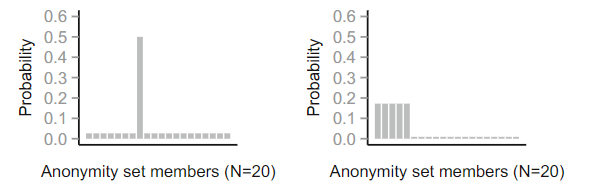
\includegraphics[scale=0.8]{pics/plot.png}
    \caption{Deux distributions\cite{anon_quantify}[9] avec la même cardinalité ($\approx$ 4.32 bits), 
    la même entropie de Shannon ($\approx$ 3.12 bits) et la même entropie normalisée 
    ($\approx$ 0.72)}
\end{figure}

La distribution de gauche a un émetteur avec une probabilité de $\frac{1}{2}$
et les 19 autres avec une probabilité de $\frac{1}{38}$.
La distribution de droite a 5 émetteurs avec une probabilité de $\frac{a}{5}$
et les 15 autres avec une probabilité de $\frac{1-a}{15}$ où $a \approx 0.86$
est la solution de l'équation définie par Toth dans \og Measuring anonymity\
revisited\fg. Un observateur capable d'enquêter uniquement un seul émetteur a une 
chance de réussite de 50\% dans la distribution de gauche et de 17.2\%
dans celle de droite. D'où l'utilisation de la min-entropie, une mesure 
conservatrice qui décrit l'imprévisibilité d'un résultat déterminé par la 
probabilité du résultat le plus probable. Cela correspond à la sécurité effective
dans le cas d'un observateur capable d'enquêter sur un seul émetteur. 
La min-entropie de la distribution de gauche est de 1 bit et celle de droite de 
$\approx$ 2.54 bits. Du point de vue du concepteur d'un système, on privilègera 
donc la distribution de droite à celle de gauche.

\begin{definition}[Min-entropie]
    $H_{min}(S) = - log_2(max \: p_i)$
\end{definition}

